\section{Vibration Acquisition Channel}\label{sec:vibration-acquisition-channel}

\subsection{Accelerometer}\label{ssec:accelerometer-signal}
	As mentioned in Section \ref{ssec:accelerometer}, acceleration is measured in g. The choosen accelerometer for this project was the \textit{ADXL335} from \textit{Analog Devices} \cite{devices2010adxl335}. The main characteristics of this sensor are:

	\begin{itemize}
		\item It has 3 axis sensing (easy to install).
		\item Low power operation (350$\micro$A).
		\item 10,000 g shock survival.
		\item 1V8-3V3 Single-supply operation.
		\item $\pm$3g measurements.
	\end{itemize}

	When powered up with 3V3 the sensor has a linear voltage output of 0V for -3g and 3V3 for 3g. This sensor is ideal for this project, the only issue is the installation. The sensor comes in a 16-LFCSP IC (Figure \ref{fig:16lfcsp}), and this IC needs to be installed where acceleration is intended to be measured, so a additional board is necessary to install it. 

	\begin{figure}[htbp]
		\centering
			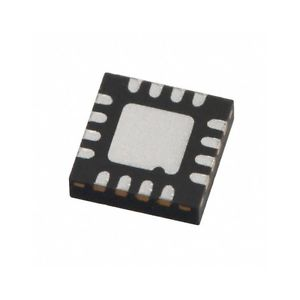
\includegraphics[scale=0.95]{figuras/fig-16lfcsp.jpg}
		\caption{16-LFCSP \cite{16lfcsp}}
		\label{fig:16lfcsp}
	\end{figure}

	The are already embdded solutions that can solve this issue, such as the \textit{Adafruit ADXL335 - 5V ready} \cite{adafruit-5v-ready}. This small (75mm x 75mm) board (Figure \ref{fig:adafruit-adxl335}) has the ADXL335 with the capacitors recommended by the datasheet, with a 3V3 voltage regulator so the board can be powererd up with 5V and with the mounting holes to fix the board in any surface, making it ideal for this project.

	\begin{figure}[htbp]
		\centering
			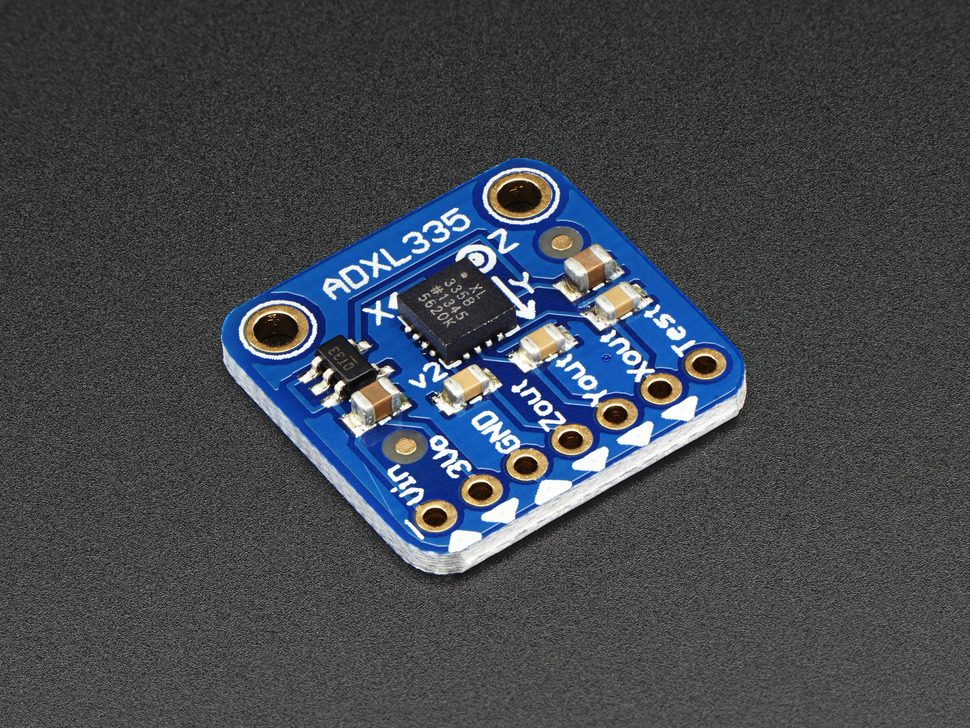
\includegraphics[scale=0.95]{figuras/fig-adafruit-adxl335.jpg}
		\caption{Adafruit ADXL335 - 5V ready \cite{adafruit-adxl335}}
		\label{fig:adafruit-adxl335}
	\end{figure}


\subsection{Signal Conditioning Circuit}\label{ssec:accelerometer-signal-conditioning-circuit}

	The ADXL335 datasheet \cite{devices2010adxl335} says that for a -3g measured acceleration the device output is of 0V and for +3g measurement it is 3V3 voltage. As said in Section \ref{ssec:the-choosen-mcu}, the choosen MCU for this project has a ADC with a 5V voltage reference, so in order to use the maximum number os bits from the ADC is it important to amplify this 0-3V3 signal to a 0-5V signal, meaning we need a circuit with a amplification gain of 1.5x.
	\par
	The sensor conditioning circuit is displayed on Figure \ref{fig:accelerometer-signal-conditioning-circuit}.

	\begin{figure}[htbp]
		\centering
			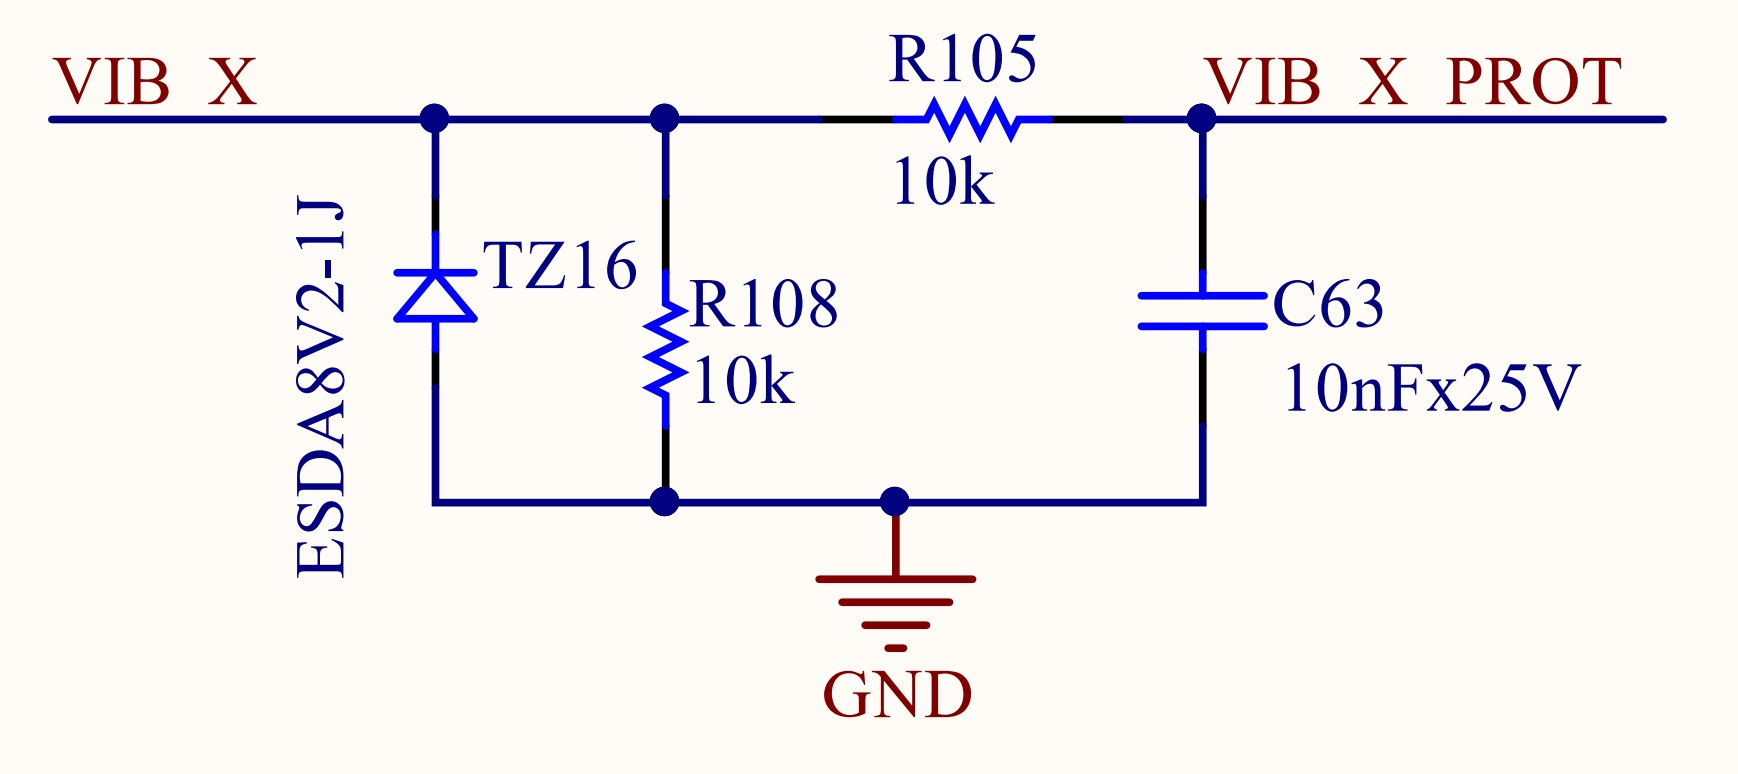
\includegraphics[scale=0.95]{figuras/fig-accelerometer-signal-conditioning-circuit.jpg}
		\caption{Accelerometer Signal Conditioning Circuit \cite{accelerometer-signal-conditioning-circuit}}
		\label{fig:accelerometer-signal-conditioning-circuit}
	\end{figure}


	The circuit is composed of three stages: protection, amplification and post-filtering. 

	\begin{itemize}
		\item \textbf{First Stage} \textit{(protection)}: Composed of a TVS diode with a standoff voltage of 3V3 (same as the sensor maximum normal output voltage level, check Item \ref{itm:tvs-standoff-voltage} from Section \ref{ssssec:tvsSelection}) and a LPF with a cutoff frequency of approximately 1.6kHz (enough to filter most ESD, check Section \ref{sssec:lowPassFilterTransientProtection}). 

		\item \textbf{Second Stage} \textit{(amplification)}: The second stage is composed by a simple non-inverting amplifier with a gain of 1.5x, to achieve this gain the resistors were choosing using Equation \ref{eqn-gain-neg-closed-loop-amp} from Section \ref{ssec:closed-loop-amplifier}. The choosen OPAMP is the \textit{MCP6001} from \textit{Microship} \cite{mcp6001-datasheet}, it was choosen for this project because it optimized to work with single-supply, has rail-to-rail input/output and has wide-bandwidth operation.

		\item \textbf{Third Stage} \textit{(post-filtering)}: The third and final stage is composed just by a LPF filter to attenuate any post amplification noise and the 50/60Hz noise interference from the power line. It has a cutoff frequency of approximately 16Hz.

	\end{itemize}

	Resistor R92 is just a jumper that was included if this circuit block is intended to be tested separately from the rest of the circuit. Resistors R96 and R94 are external pull-downs and in theory should not be mounted, they were included in the layout just in case this pull-downs become needed and then a new PCB layout would not be necessary. Capacitor C43 is just a decoupling capacitor for the amplifier supply recommended by the component datasheet \cite{mcp6001-datasheet}.

\subsection{Sensor Detection Circuit}\label{ssec:accelerometer-sensor-detection-circuit}

	As mentioned in Section \ref{ssec:accelerometer-signal}, the choosen solution for the accelerometer \textit{(Adafruit ADXL335 - 5V ready)} has a integrated 3V3 voltage regulator. In Figure \ref{fig:adafruit-adxl335} it is possible to see that the 3V3 voltage output from the voltage regulator has a connection point on the board. Hence, if a wire is connected to this point and to the main circuit board, whenever this point does not have 3V3 voltage the sensor is disconnected. Moreover, the detection circuit just need to detect when the line is in 0V or 3V3.